\documentclass{beamer}
\mode<presentation>
\usepackage{amsmath}
\usepackage{amssymb}

%\usepackage{advdate}
\usepackage{adjustbox}
\usepackage{subcaption}
\usepackage{enumitem}
\usepackage{multicol}
\usepackage{mathtools}
\usepackage{listings}
\usepackage{url}
\usepackage{xcolor}
\def\UrlBreaks{\do\/\do-}
\usetheme{Boadilla}
\usecolortheme{lily}
\setbeamertemplate{footline}
{
  \leavevmode%
  \hbox{%
  \begin{beamercolorbox}[wd=\paperwidth,ht=2.25ex,dp=1ex,right]{author in head/foot}%
    \insertframenumber{} / \inserttotalframenumber\hspace*{2ex} 
  \end{beamercolorbox}}%
  \vskip0pt%
}
\setbeamertemplate{navigation symbols}{}

\providecommand{\nCr}[2]{\,^{#1}C_{#2}} % nCr
\providecommand{\nPr}[2]{\,^{#1}P_{#2}} % nPr
\providecommand{\mbf}{\mathbf}
\providecommand{\pr}[1]{\ensuremath{\Pr\left(#1\right)}}
\providecommand{\qfunc}[1]{\ensuremath{Q\left(#1\right)}}
\providecommand{\sbrak}[1]{\ensuremath{{}\left[#1\right]}}
\providecommand{\lsbrak}[1]{\ensuremath{{}\left[#1\right.}}
\providecommand{\rsbrak}[1]{\ensuremath{{}\left.#1\right]}}
\providecommand{\brak}[1]{\ensuremath{\left(#1\right)}}
\providecommand{\lbrak}[1]{\ensuremath{\left(#1\right.}}
\providecommand{\rbrak}[1]{\ensuremath{\left.#1\right)}}
\providecommand{\cbrak}[1]{\ensuremath{\left\{#1\right\}}}
\providecommand{\lcbrak}[1]{\ensuremath{\left\{#1\right.}}
\providecommand{\rcbrak}[1]{\ensuremath{\left.#1\right\}}}
\theoremstyle{remark}
\newtheorem{rem}{Remark}
\newcommand{\sgn}{\mathop{\mathrm{sgn}}}
\providecommand{\abs}[1]{\left\vert#1\right\vert}
\providecommand{\res}[1]{\Res\displaylimits_{#1}} 
\providecommand{\norm}[1]{\lVert#1\rVert}
\providecommand{\mtx}[1]{\mathbf{#1}}
\providecommand{\mean}[1]{E\left[ #1 \right]}
\providecommand{\fourier}{\overset{\mathcal{F}}{ \rightleftharpoons}}
%\providecommand{\hilbert}{\overset{\mathcal{H}}{ \rightleftharpoons}}
\providecommand{\system}{\overset{\mathcal{H}}{ \longleftrightarrow}}
	%\newcommand{\solution}[2]{\textbf{Solution:}{#1}}
%\newcommand{\solution}{\noindent \textbf{Solution: }}
\providecommand{\dec}[2]{\ensuremath{\overset{#1}{\underset{#2}{\gtrless}}}}
\newcommand{\myvec}[1]{\ensuremath{\begin{pmatrix}#1\end{pmatrix}}}
\let\vec\mathbf

\lstset{
%language=C,
frame=single, 
breaklines=true,
columns=fullflexible
}

\numberwithin{equation}{section}

\title{10.3.6.1.8}
\author{Sruthi B \\ EE24BTECH11060\\}

\date{\today} 
\begin{document}
\begin{frame}
\titlepage
\end{frame}

\section*{Outline}
\begin{frame}
\tableofcontents
\end{frame}
\section{Problem}
\section{Numerical methods}
\section{FIGURE}

\begin{frame}
   \frametitle{PROBLEM STATEMENT}
Solve the following pairs of equations by reducing them to a pair of linear equations:
\begin{align*}
    \frac{1}{3x+y} + \frac{1}{3x-y} &= \frac{3}{4}\\
    \frac{1}{2\brak{3x+y}} - \frac{1}{2\brak{3x-y}} &= \frac{-1}{8}
\end{align*}
\end{frame}
\begin{frame}
\frametitle{Numerical Method}
 Let's solve this using LU decomposition. First, let's substitute:
\begin{align}
    \frac{1}{3x+y} &= u\\
    \frac{1}{3y-y} &= v
\end{align}

Then our equations become:
\begin{align}
    u + v &= \frac{3}{4} \label{eq1}\\
    \frac{1}{2}u - \frac{1}{2}v &= \frac{-1}{8} \label{eq2}
\end{align}
\begin{align}
    4u + 4v &= 3 \label{eq1}\\
    4u - 4v &= -1 \label{eq2}
\end{align}
This can be written in matrix form as:
\begin{align}
    \myvec{4 & 4 \\ 4& -4}\myvec{u\\v} = \myvec{3\\-1}
\end{align}
\end{frame}
\begin{frame}
\frametitle{Numerical Method}
 Let A=$\myvec{4 & 4 \\ 4& -4}$\\
By multiplying A on both sides\\
\begin{align}
    \myvec{4 & 4 \\ 4& -4}\myvec{4 & 4 \\ 4& -4}\myvec{u\\v} = \myvec{4 & 4 \\ 4& -4}\myvec{3\\-1}
\end{align}
after solving 
\begin{align}
    \myvec{u\\v}=\myvec{\frac{1}{4}\\ \frac{1}{2}}
\end{align}
Therefore:
\begin{align}
    \frac{1}{3x+y} =\frac{1}{4} &\implies 3x+y=4\\
    \frac{1}{3x-y} = \frac{1}{2} &\implies 3x-y =2\\
\end{align}

\end{frame}
\begin{frame}
\frametitle{Numerical Method}
Any non-singular matrix can be represented as a product of a lower triangular matrix $L$ and an upper triangular matrix $U$
\begin{align}
	\vec{A}\vec{x} = \vec{L}\vec{U}\vec{x} = \vec{b}
\end{align}
\textbf{Factorization of LU:}\\
Given a matrix $ \mathbf{A} $ of size $ n \times n $, LU decomposition is performed row by row and column by column. The update equations are as follows: 
\begin{itemize}
    \item Start by initializing $ \mathbf{L} $ as the identity matrix $ \mathbf{L} = \mathbf{I} $ and $ \mathbf{U} $ as a copy of $ \mathbf{A} $.\\
    \item For each column $ j \geq k $, the entries of $ U $ in the $ k $-th row are updated as:
    \begin{align}
        U_{k,j} = A_{k,j} - \sum_{m=1}^{k-1} L_{k,m} \cdot U_{m,j}\quad \forall \quad j \geq k
    \end{align}
    \end{itemize}
\end{frame}
\begin{frame}
\frametitle{Numerical Method}
\begin{itemize}
\item For each row $ i > k $, the entries of $ L $ in the $ k $-th column are updated as:
    \begin{align}
        L_{i,k} = \frac{1}{U_{k,k}} \brak{ A_{i,k} - \sum_{m=1}^{k-1} L_{i,m} \cdot U_{m,k}} \quad \forall \quad i > k
    \end{align}
    \end{itemize}
    By doing the following steps and solving we get :
\begin{align}
    \myvec{3 & 1 \\ 3& -1}\myvec{x\\y} = \myvec{4\\2}
\end{align}
By doing the following factorization we get:
\begin{align}
	\vec{U}=\myvec{3 & 1\\0 & -2} and  \vec{ L} = \myvec{1 & 0\\ 1 & 1}
\end{align}
We can solve this using two steps:
\begin{align}
    L\vec{y} = \vec{b}\\
    U\vec{x} = \vec{y}
\end{align}
Using forward substitution:
\end{frame}
\begin{frame}

\begin{align}
    \myvec{1 & 0\\ 1 & 1}\myvec{y_1\\y_2} = \myvec{4\\2}\\
    \implies y_1 =4\\
    \implies y_2 =-2
\end{align}
Now using back substitution:
\begin{align}
    \myvec{3 & 1\\0 & -2}\myvec{x\\y} = \myvec{4\\ -2}
\end{align}

This gives:
\begin{align}
      \implies y&=1\\
    3x + 1 &= 4\\
    x &= 1
\end{align}

The solution is:
\begin{align}
    \myvec{x\\y} = \myvec{1 \\ 1}
 \end{align}
\end{frame}
\begin{frame}
\frametitle{Figure}
\begin{figure}[h!]
   \centering
	 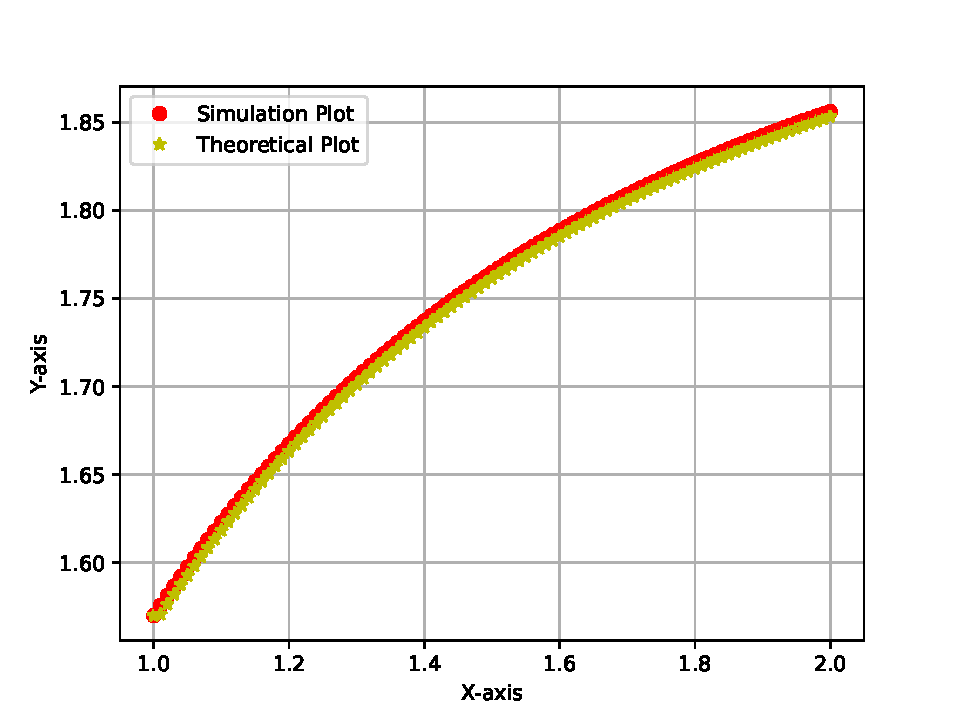
\includegraphics[width=0.8\textwidth]{fig.pdf}
   % Add your figure here if needed
\end{figure}

\end{frame}

\end{document} 
